\documentclass{article}
\usepackage{graphicx}
\usepackage{amsmath}
\usepackage{float}
\usepackage{wrapfig}
\usepackage{tcolorbox}
\usepackage{lipsum}


\begin{document}
	\begin{titlepage}

	\title{Autonomus Surface Oceanographer}
	\author{Attila Fodor \\\\ Department of Automation and Applied Informatics\\
Budapest University of Technology and Economics\\
Budapest, Hungary}

	\maketitle
	\thispagestyle{empty}

	\begin{abstract}
		The document introduces the reader to the world of seaborne measurements, and proposes a new way of 		oceanography, by centering around the concept of an Autonomous Surface Oceanographer. Each paragraph 		follows through a special part of the complex oceanography task, in order to give an overview about 		the challenges of the science crew, while explaining the various stages of development associated to 		that specific stage of action.
	\end{abstract}

\end{titlepage}

%\chapter*{Introduction}\addcontentsline{toc}{chapter}{Introduction}
\section{Introduction}

Seaborne measurements are often expensive and time consuming, though they can have a large impact on the area, where the data have been obtained. In 2011 the naval safe zone around the Fukusima accident was laid down based only on estimates of the radiation contamination\cite{FNPP}, because low amount of measurement data was available due to high measurement costs and risks. Another notable example are the coastal waters of Greenland, because are very poorly mapped up to present day\cite{2009AGUFMOS21A1152W}. Ships have to sail in a roundabout way around the island, because the risk of wrecking in unknown fjordic area is very high. This is a huge waste of time and natural resources annually.

\subsection*{Oceanography and Bathymetry}

Not many people come across these expressions often. Oceanography can be summarized as a branch of Earth science that studies the ocean. It includes a wide range of topics, like the study of marine ecosystem, ocean currents, plate tectonics and the geology of the sea floor. Bathymetry is the study of underwater depth of lake or ocean floors. The advancing technology allows even more possibilities, like the aforementioned radiological measurements, or general monitoring of the seas.

\subsection{Advantages of autonomous vessels}

Oceanographic measurements today are carried out by large crewed ships, but in many cases they could be replaced by a number of smaller crafts, in order to reduce surveying time and cost and increase the available manpower in other tasks. These vessels could have the ability to sail previously unsurveyable areas as well, thanks to the shallower draught and smaller size.

\subsection{Limitations}

The most notable limitation of the current mobile robotic technologies are their small size itself. It means the relatively small range based on their smaller power capabilities, and narrow field of application.

The aim of this project is to develop an autonomous surface vehicle, which is capable of conducting multiple seaborne measurements. To execute an oceanography mission, the ship must be capable of autonomus navigation based on Global Positioning System (GPS) and an Internal Measurement Unit (IMU), to further enhance the precision in hazardous environment.

\begin{figure}[H]
	\centering
	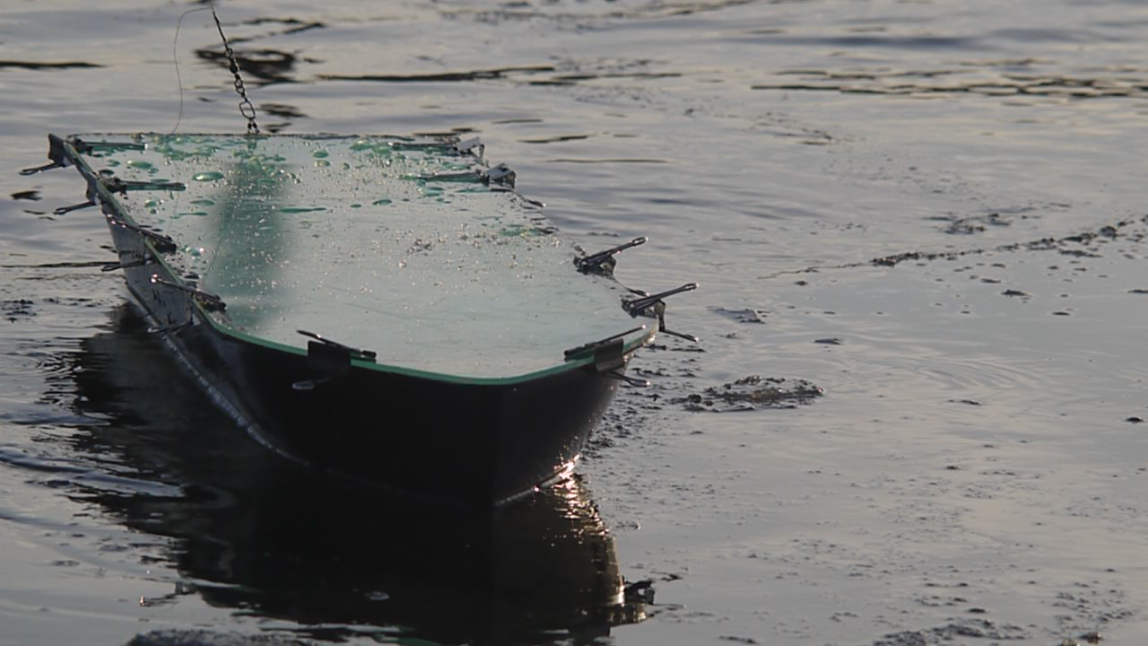
\includegraphics[width=0.8\textwidth]{img/aauship}
	\caption{The AAUSHIP prototype on her maiden voyage}
	\label{fig:aauship}
\end{figure}

\subsection*{Development guidelines}
In order to keep a sensible and extendable system, the control software of the ship follows the guidelines of the Model-Based Design approach. The system software can be divided to two different kind of modules, one that is dependent, and one that is independent from the physical characteristics of the vessel. In order to maximize the extendability of the system, the fix (independent) modules must be completely general, but as thorough as possible, so as to keep the complexity of the changeable (dependent) software of the robot minimal.
\begin{wrapfigure}{r}{0.48\textwidth}
  \begin{center}
    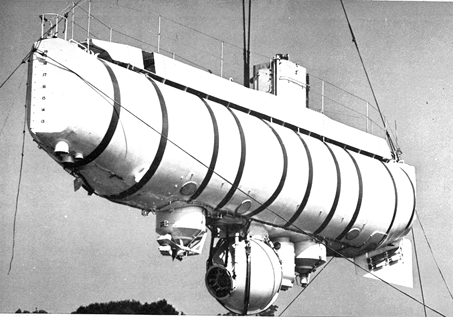
\includegraphics[width=0.5\textwidth]{img/trieste}
  \end{center}
  \caption{Bathyscaphe Trieste, the first manned vessel that reached the bottom of Challenger Deep (Mariana Trench)\cite{trieste}}
\end{wrapfigure}

The environment stored in the control system must be extendable to the third dimension, and must be able to track changes over time.
The tasks of the low level control must be as specific and as basic as possible. All calculations and control should be implemented in the high level controller.
the high level controller must be parametrized, based on the low level and hardware characteristics.

The point of these guidelines is to create a system of components with major reusability. Ideally a general Cross-platform High Level Controller controls different kind of vessels, through a standard interface. When changing to an arbitrary different vehicle, only the Low Level Controller must be replaced, which stores the characteristics of the vessel and implements the actuator control.

\section*{Operation models}

 A typical oceanography application starts on the shore. A science team analyzes the currently available data, then marks the area of measurements on the map. The  map data is transformed to a measurement path by the scientists or by the automatic waypoint planner of the ship. The autonomous surface vehicle is then outfitted with the right sensors for the task, and a manned ship transports it close to its destination. The crew can set the research vessel to manual, automatic or fully autonomous mode.

\paragraph{Manual control}
In this mode it's possible for the operator to control the movement of the ship, degree of freedom-wise or control the actuators themselves. The primary intent of this mode is for testing or malfunction-recovery.

\begin{figure}[H]
	\centering
	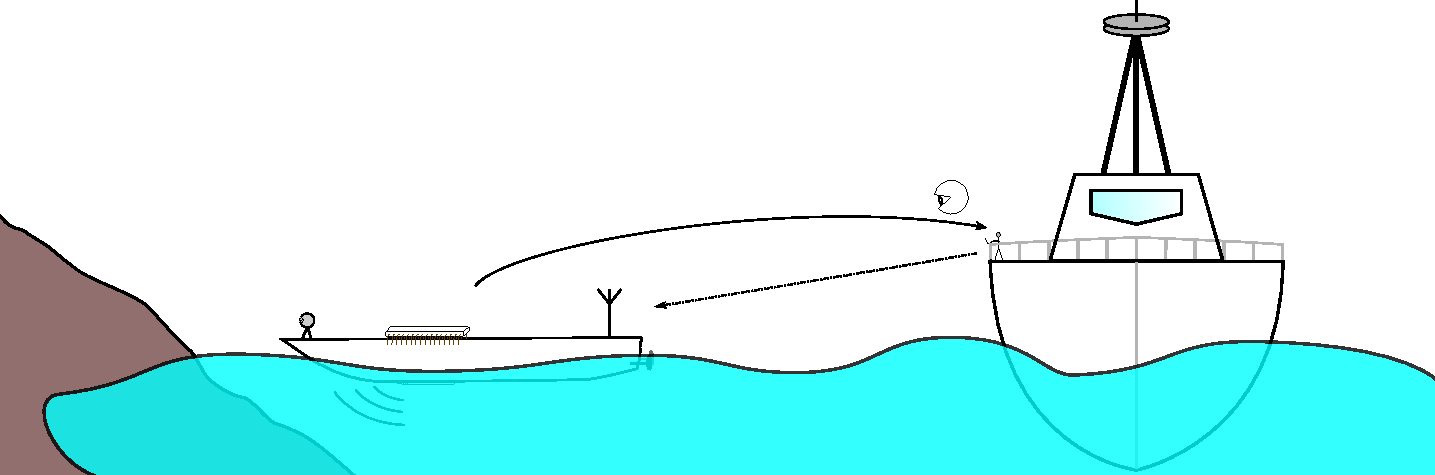
\includegraphics[width=0.8\textwidth]{img/manualcontrol}
	\caption{Manual remote control}
	\label{fig:manualcontrol}
\end{figure}

\paragraph{Automatic control}
In automatic mode the "brains", remain on the crewed vessel, and the research craft remains in wireless connection with the Mothership. When the measurements are complete, the oceanographer returns to the mothership. In automatic mode it is always possible to switch to manual control and back, or update the measurement path, etc.

\begin{figure}[H]
	\centering
	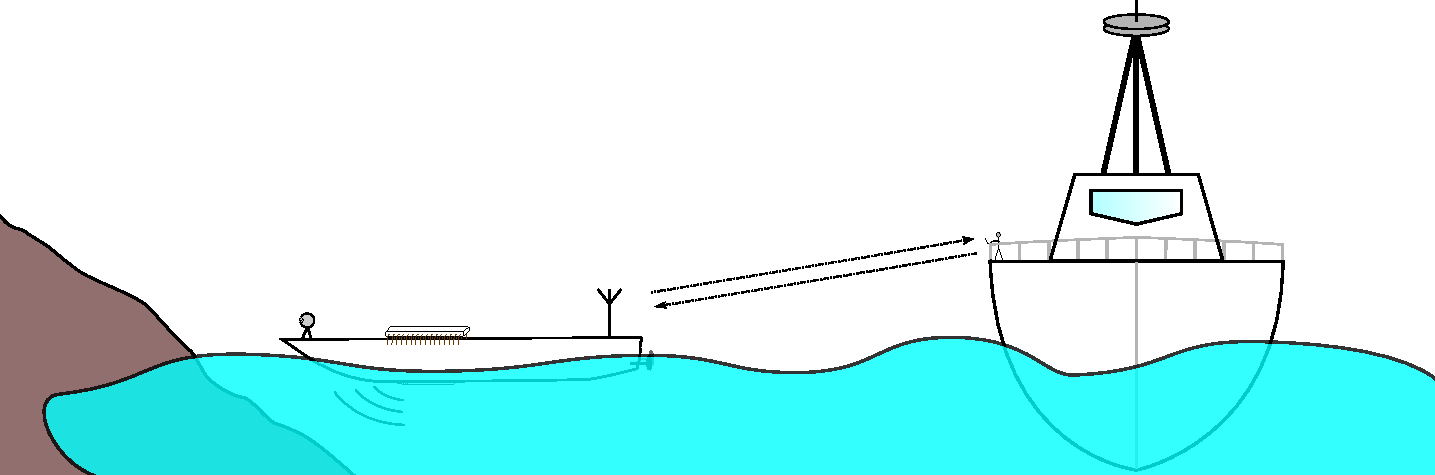
\includegraphics[width=0.8\textwidth]{img/automatic}
	\caption{Automatic supervised control}
	\label{fig:automatic}
\end{figure}

\paragraph{Autonomus control}
In Autonomus mode the ship carries everything that is needed to complete the task. Connection to the mothership can be cut, and the vessel carries the orders out autonomusly. Intervention in this mode is only possible until the oceanographer is in range of the mothership.

\begin{figure}[H]
	\centering
	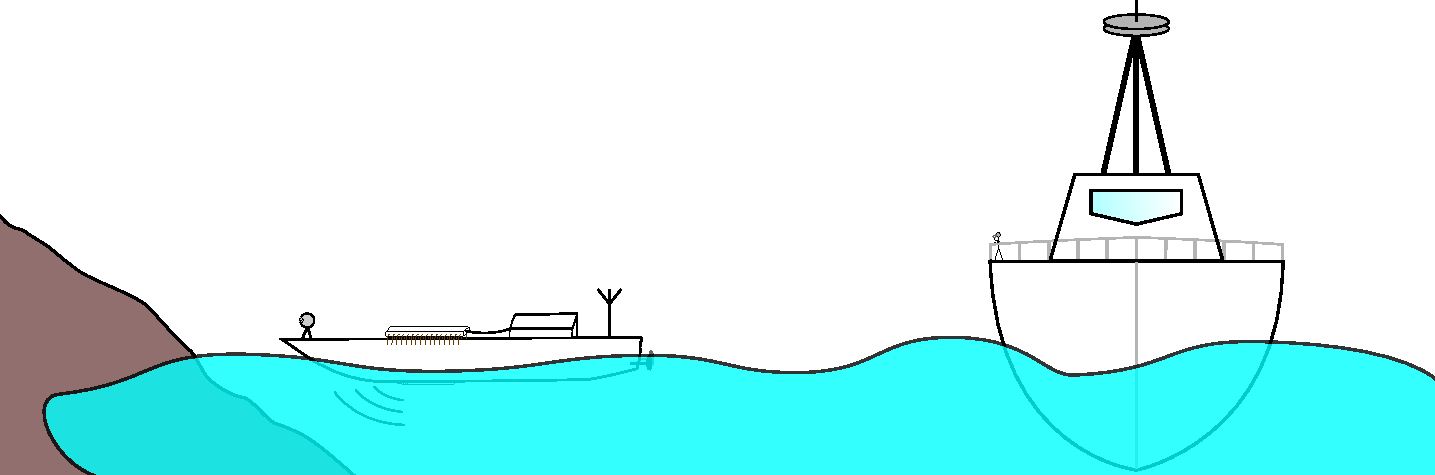
\includegraphics[width=0.8\textwidth]{img/autonomus}
	\caption{Autonomus control}
	\label{fig:autonomus}
\end{figure}

\paragraph{}
In case there are multiple research vessels, they can form a squadron. In this setup only one of the ships needs to be in range of the crewed mothership. Alternatively one autonomus ship is capable of controlling multiple automatic crafts, taking over the role of the mothership.

\begin{figure}[H]
	\centering
	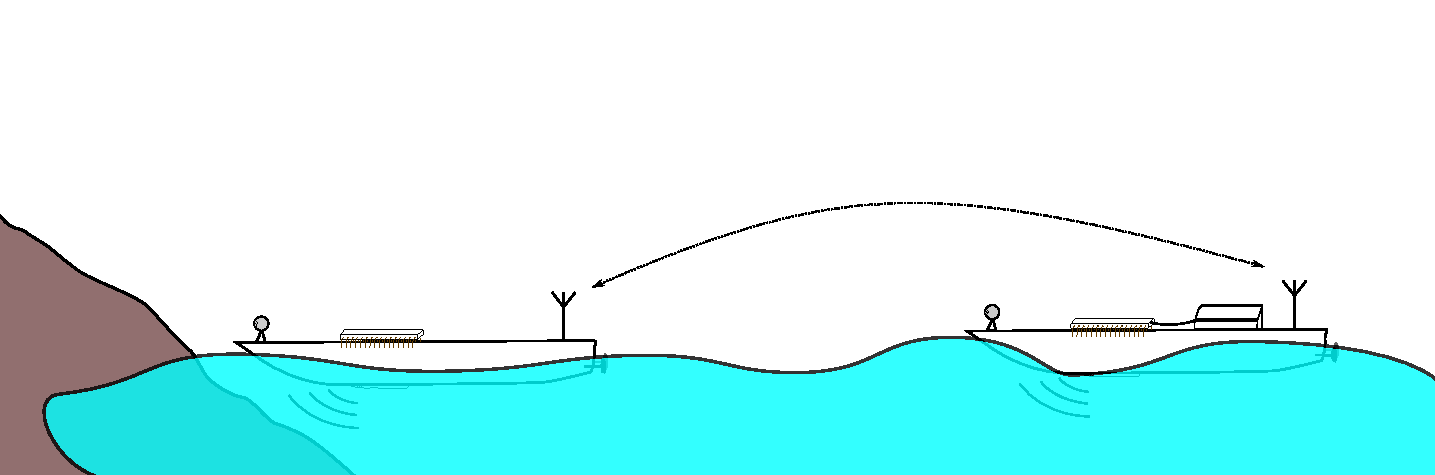
\includegraphics[width=0.8\textwidth]{img/multiple}
	\caption{Squadron mode}
	\label{fig:multiple}
\end{figure}

\begin{tcolorbox}[colback=cyan!5,colframe=cyan!40!black,title=Code: Main.py \\ https://www.dropbox.com/s/h1067ywmdajkegk/Main.py]
\begin{minipage}{0,6\textwidth}
The mission planning steps are implemented in Main.py, which is the main part of the program, responsible for initializing the system, setting the target area, mode of routing, navigation, etc. Later Main.py will provide a Graphical User Interface as well.
\end{minipage}
\begin{minipage}{0,35\textwidth}
\raggedleft

\includegraphics[width=0.8\textwidth]{img/main}
\end{minipage}

\end{tcolorbox}


\section{Pathplanning} 

The first part of the document will lay down the basic concepts and requirements of an oceanography task, focusing on the development of the High Level Controller and a seamless simulator to evaluate the results.

\subsection{Map reading}

The main method of navigation is via GPS and known shoreline database. The ship must be outfitted with proximity sensors later, in order to ensure safe navigation through traffic. During the simulation a reference shore is being generated that simulates a typical fjordic environment: Figure~\ref{fig:linemap}. The map generator is using Random Walk Functions to generate the coastline(s).

\begin{figure}[H]
	\centering
	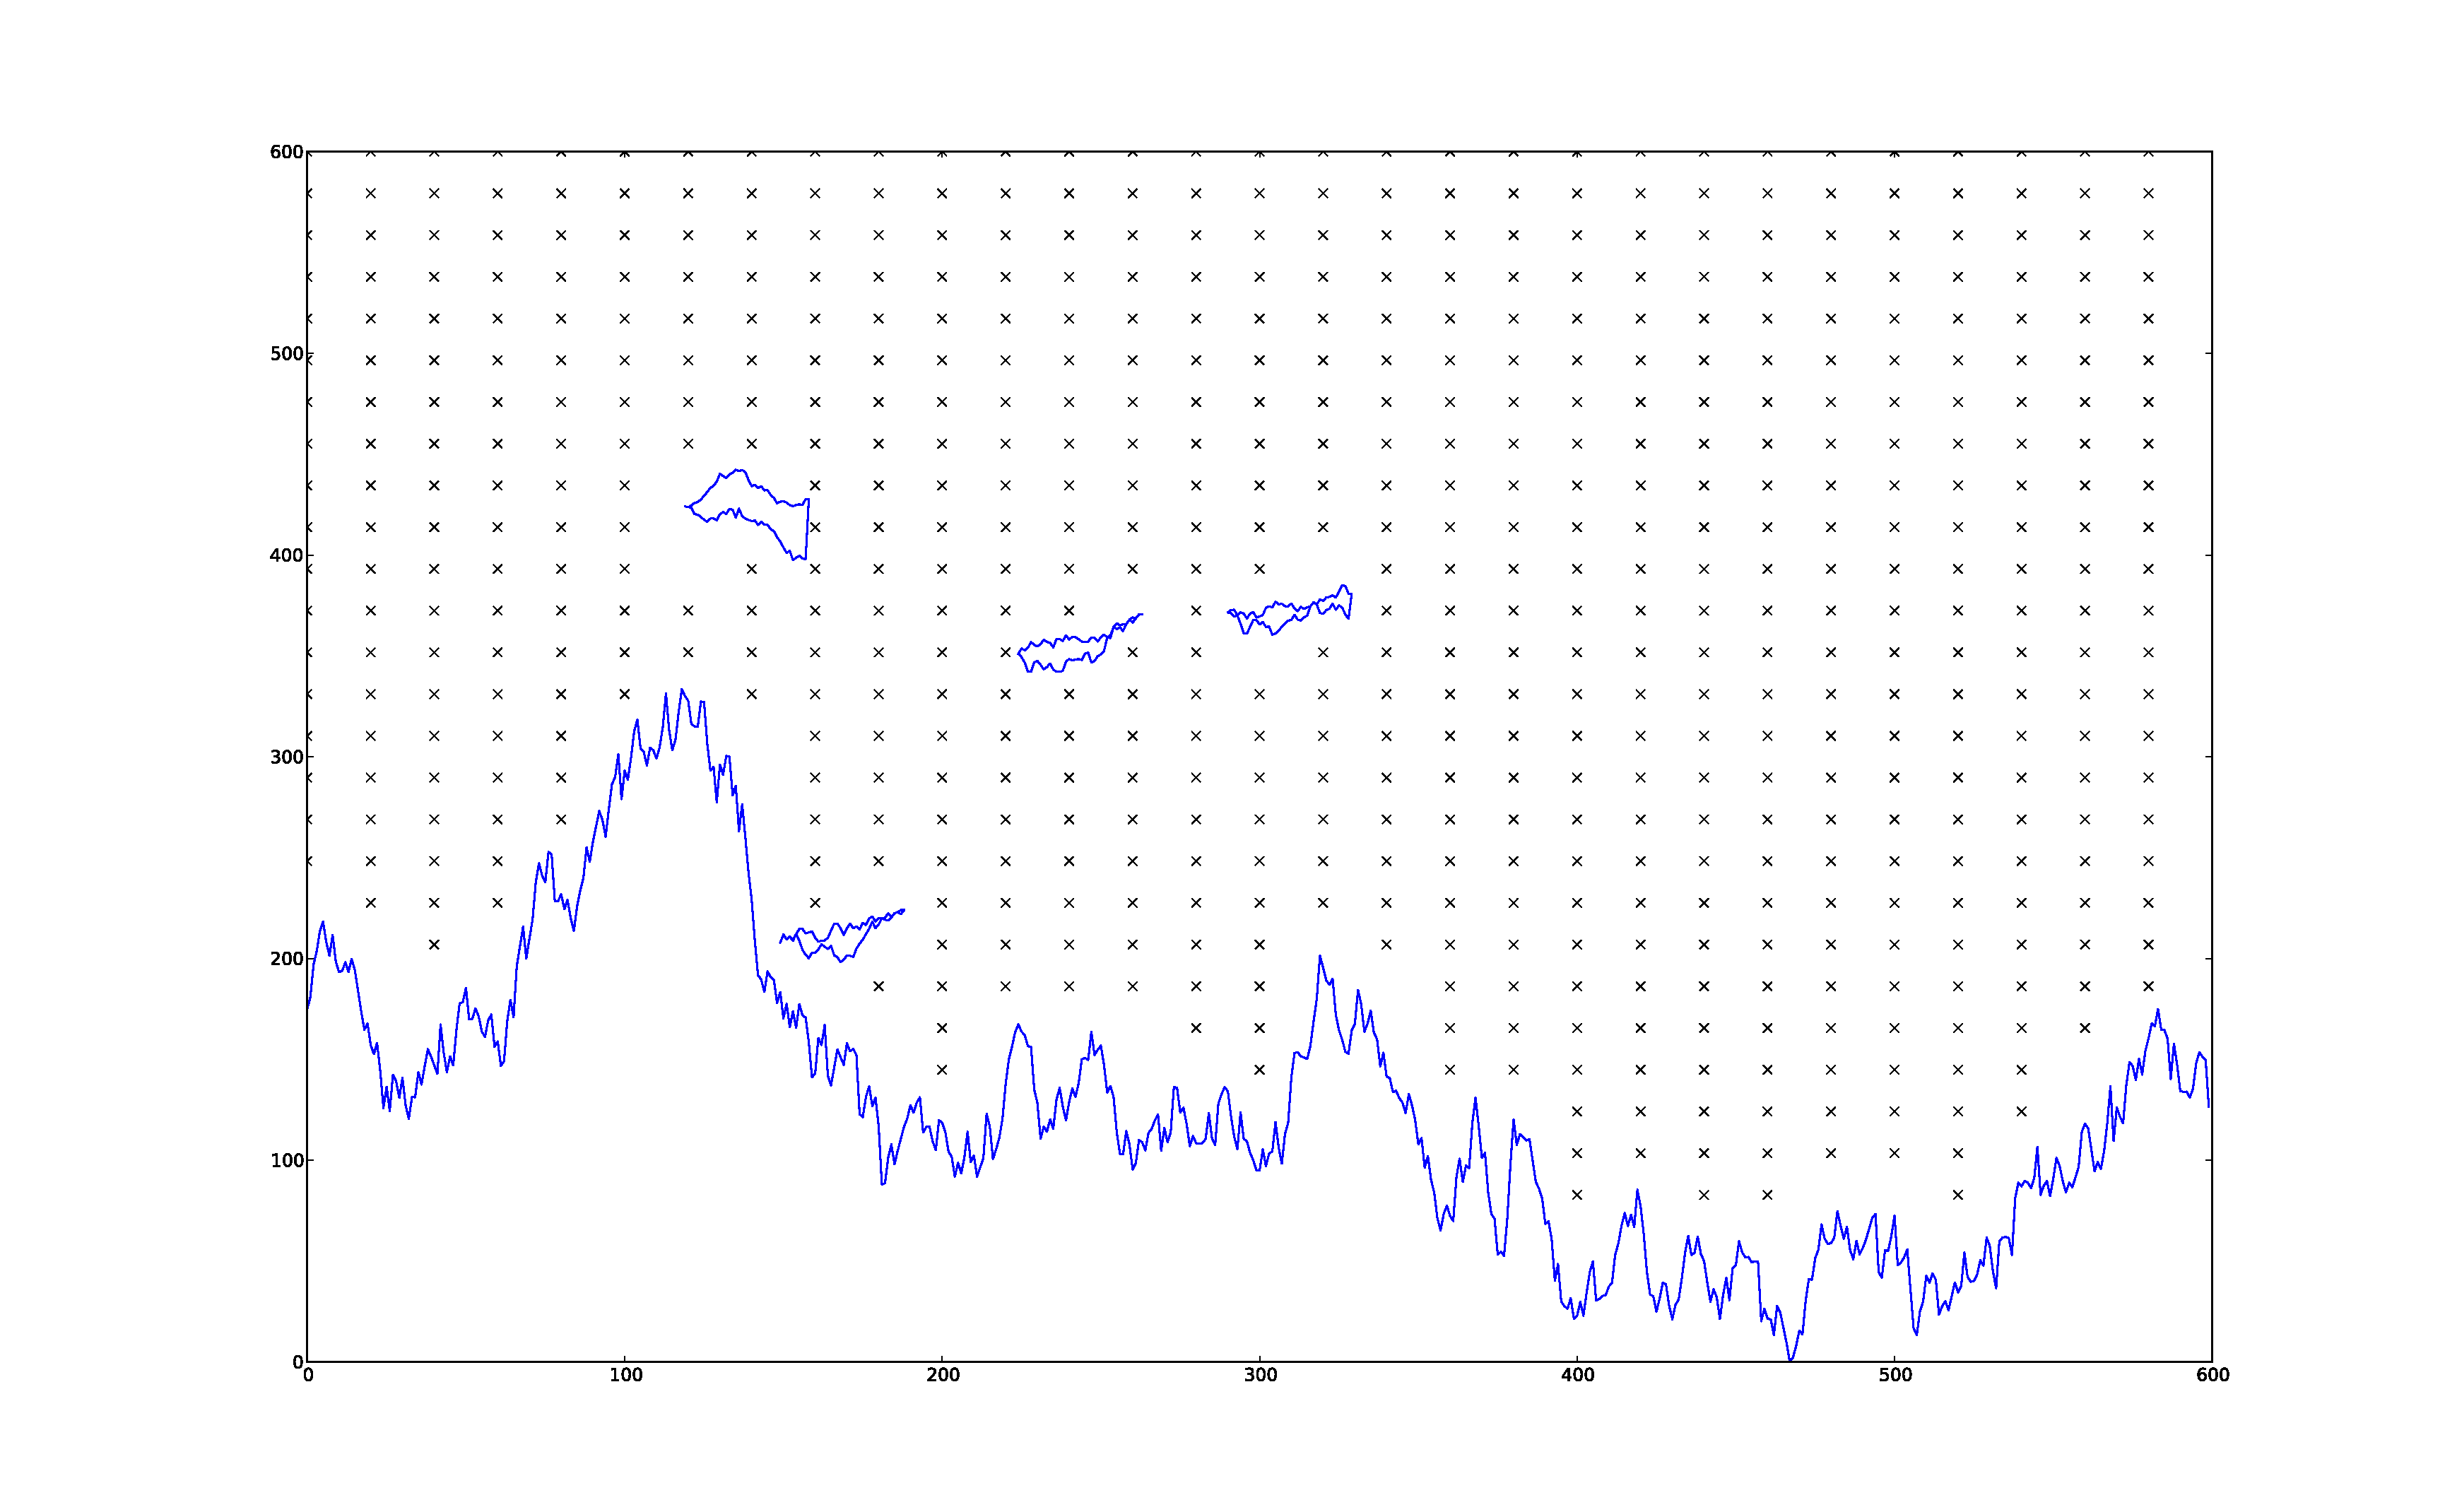
\includegraphics[width=0.8\textwidth]{img/linemap}
	\caption{The coastlines}
	\label{fig:linemap}
\end{figure}

The generated coastlines are converted to the actual Map, which is a number of surfaces: Figure~\ref{fig:solidmap}.

\begin{figure}[H]
	\centering
	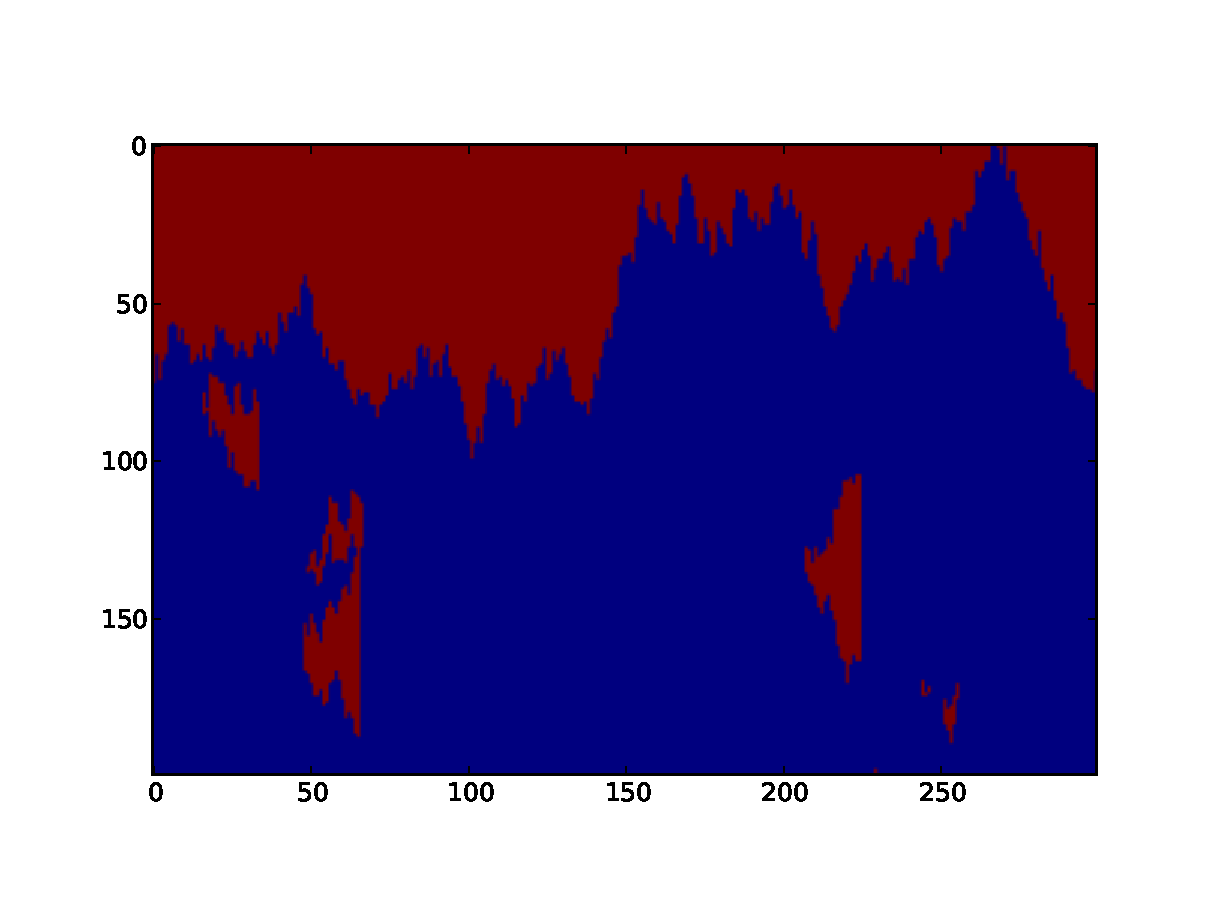
\includegraphics[width=\textwidth]{img/solidmap}
	\caption{The solidified map (the picture shows a north ("upside down") coast)}
	\label{fig:solidmap}
\end{figure}

Reading a solid map is possible from image files as well, using the Python SciPy library

\begin{figure}[H]
	\centering
	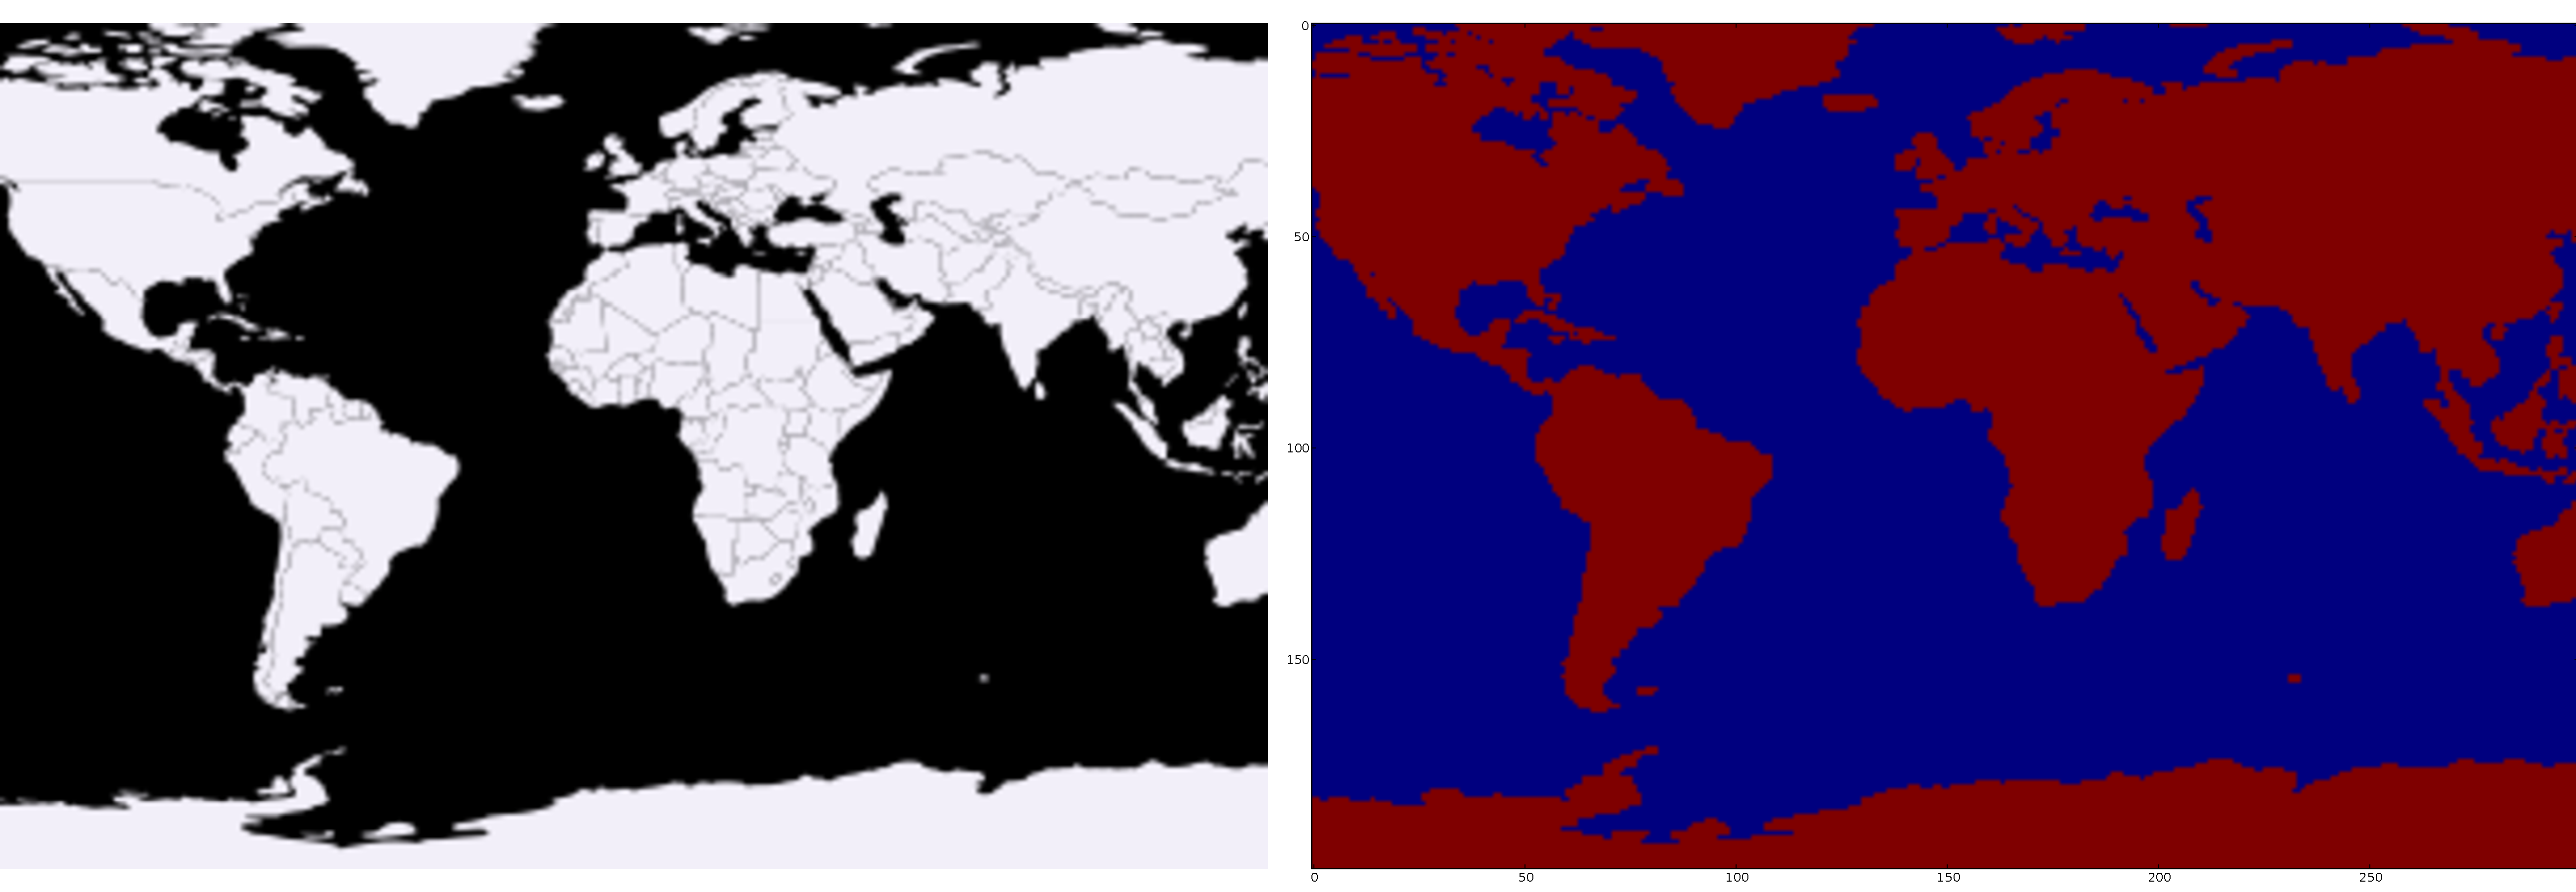
\includegraphics[width=0.8\textwidth]{img/worldmap}
	\caption{Image file processed to Map object}
	\label{fig:worldmap}
\end{figure}

\section{Routing}

Upon entering the water, the first task of the vessel in automatic or autonomus mode is to determine the course. Currently the software can not handle rivers, strong wind and magnetic declination, therefore the course is assumed to be identical to the heading.

\paragraph{The Waypoint planner} is responsible for the generating and ordering of the key measurement points. Visiting a set of waypoints on a given map leads to the Traveling Salesman NP-complete problem. Even using dynamic programming, determining the best route with the Held-Karp algorithm the program requires $O(N^2 2^2)$ steps [wiki]. The problem has been in the crosshair of mathematics for a long time, but a fast exact solution has never been found. The waypoint-planning is not time-critical, but a sufficient length of path should be calculated in a reasonable amount of time.

Fortunately the arrangement of the measurement points is relatively dense and predictable, allows only neighboring travels and repeated visits. In order to reach a suitable algorithm, some heuristics of the path planning needs to be examined.
\\

\begin{tcolorbox}[colback=cyan!5,colframe=cyan!40!black,title=Code: Ship.py \\ https://www.dropbox.com/s/fmtsaatql7jqjhw/Ship\texttt{\_}nofilter.py]
\begin{minipage}{0,6\textwidth}
Ship.py implements the Ship Object. Everything related to the handling of a ship is encapsulated in a Ship instance. Multiple instances can be created based on the same object, with different parameters, and they are using the same resources.
\end{minipage}
\begin{minipage}{0,35\textwidth}
\raggedleft

\includegraphics[width=0.8\textwidth]{img/ship}
\end{minipage}
\end{tcolorbox}

\paragraph{In a simple coastline} the points can be placed in a certain order relative to the coast, to achieve a sufficient result. If the shore is relatively smooth, the ship can also travel parallel to the coast, to decrease the required number of turns.

\begin{figure}[H]
	\centering
	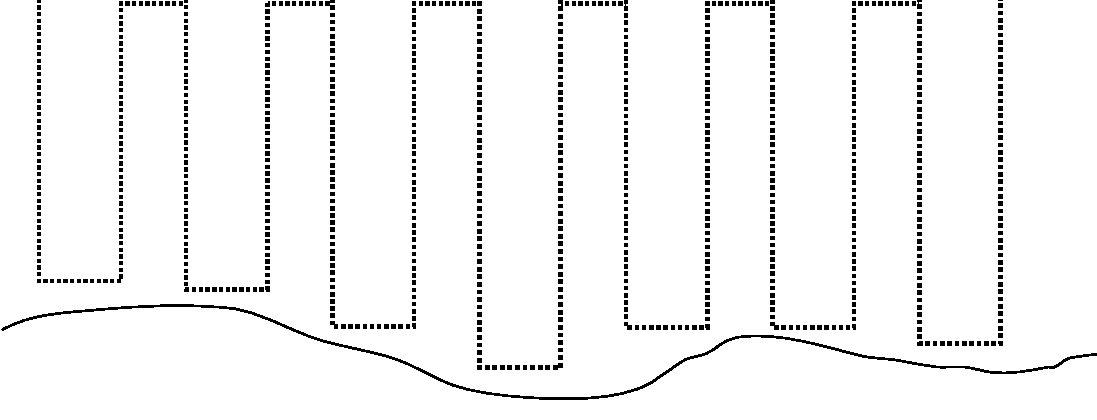
\includegraphics[width=\textwidth]{img/simplecoast}
	\caption{A simple coast and a sufficient path}
	\label{fig:simplecoast}
\end{figure}

\paragraph{Introducing isles and deep bays} to the area complicate the situation. Some waypoints need to be removed, and an avoiding path needs to be taken. This will cause many redundant measurements and very sub-optimal path, if the island density and the complexity of the coast is high.

\begin{figure}[H]
	\centering
	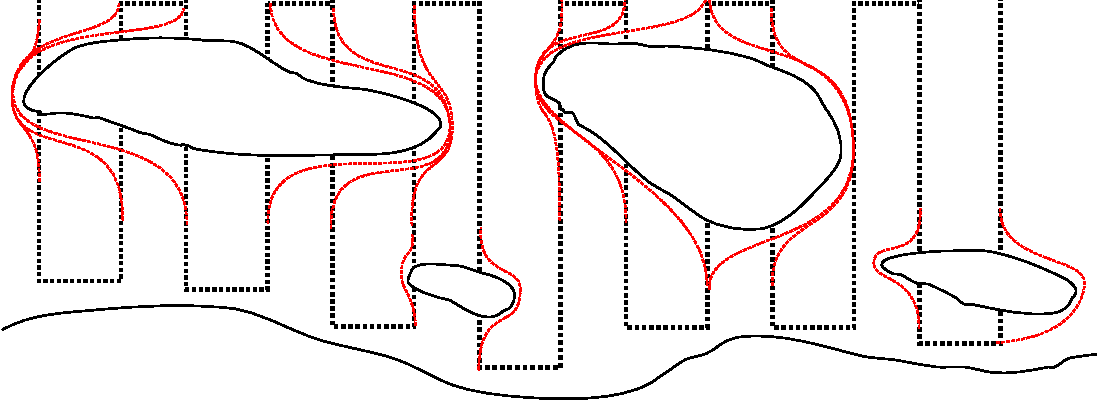
\includegraphics[width=\textwidth]{img/pathislands}
	\caption{Coast with islands}
	\label{fig:pathislands}
\end{figure}

\paragraph{Greedy traversal}

stretches a measurement grid over the area, and the points are traversed in an unpredictable way, using a neirest neighbourgh algorithm.

\begin{figure}[H]
	\centering
	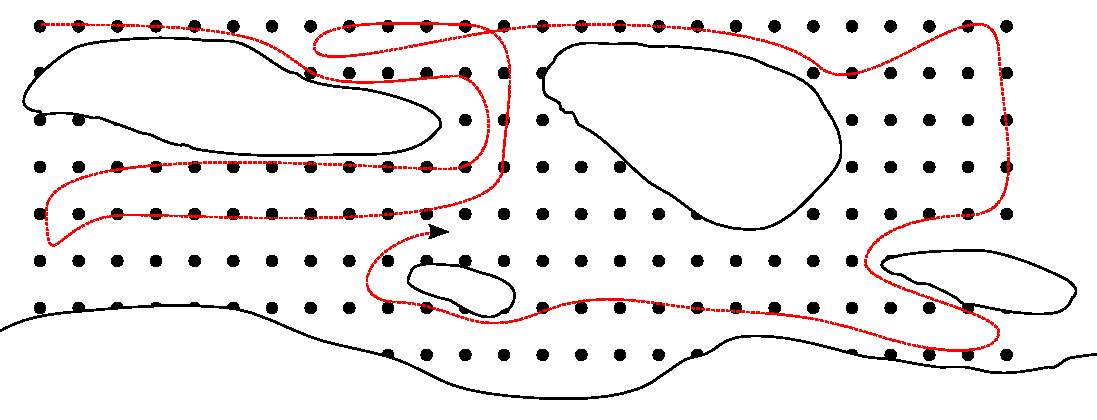
\includegraphics[width=\textwidth]{img/traversal}
	\caption{A random path based on graph traversal}
	\label{fig:traversal}
\end{figure}

 According to [citation] heuristic closest neighbour search is usually 5-10\% worse than the ideal solution. Using the closest neighbour heuristic, the simulation leads to the following path: Figure~\ref{fig:nn}.

\begin{figure}[H]
	\centering
	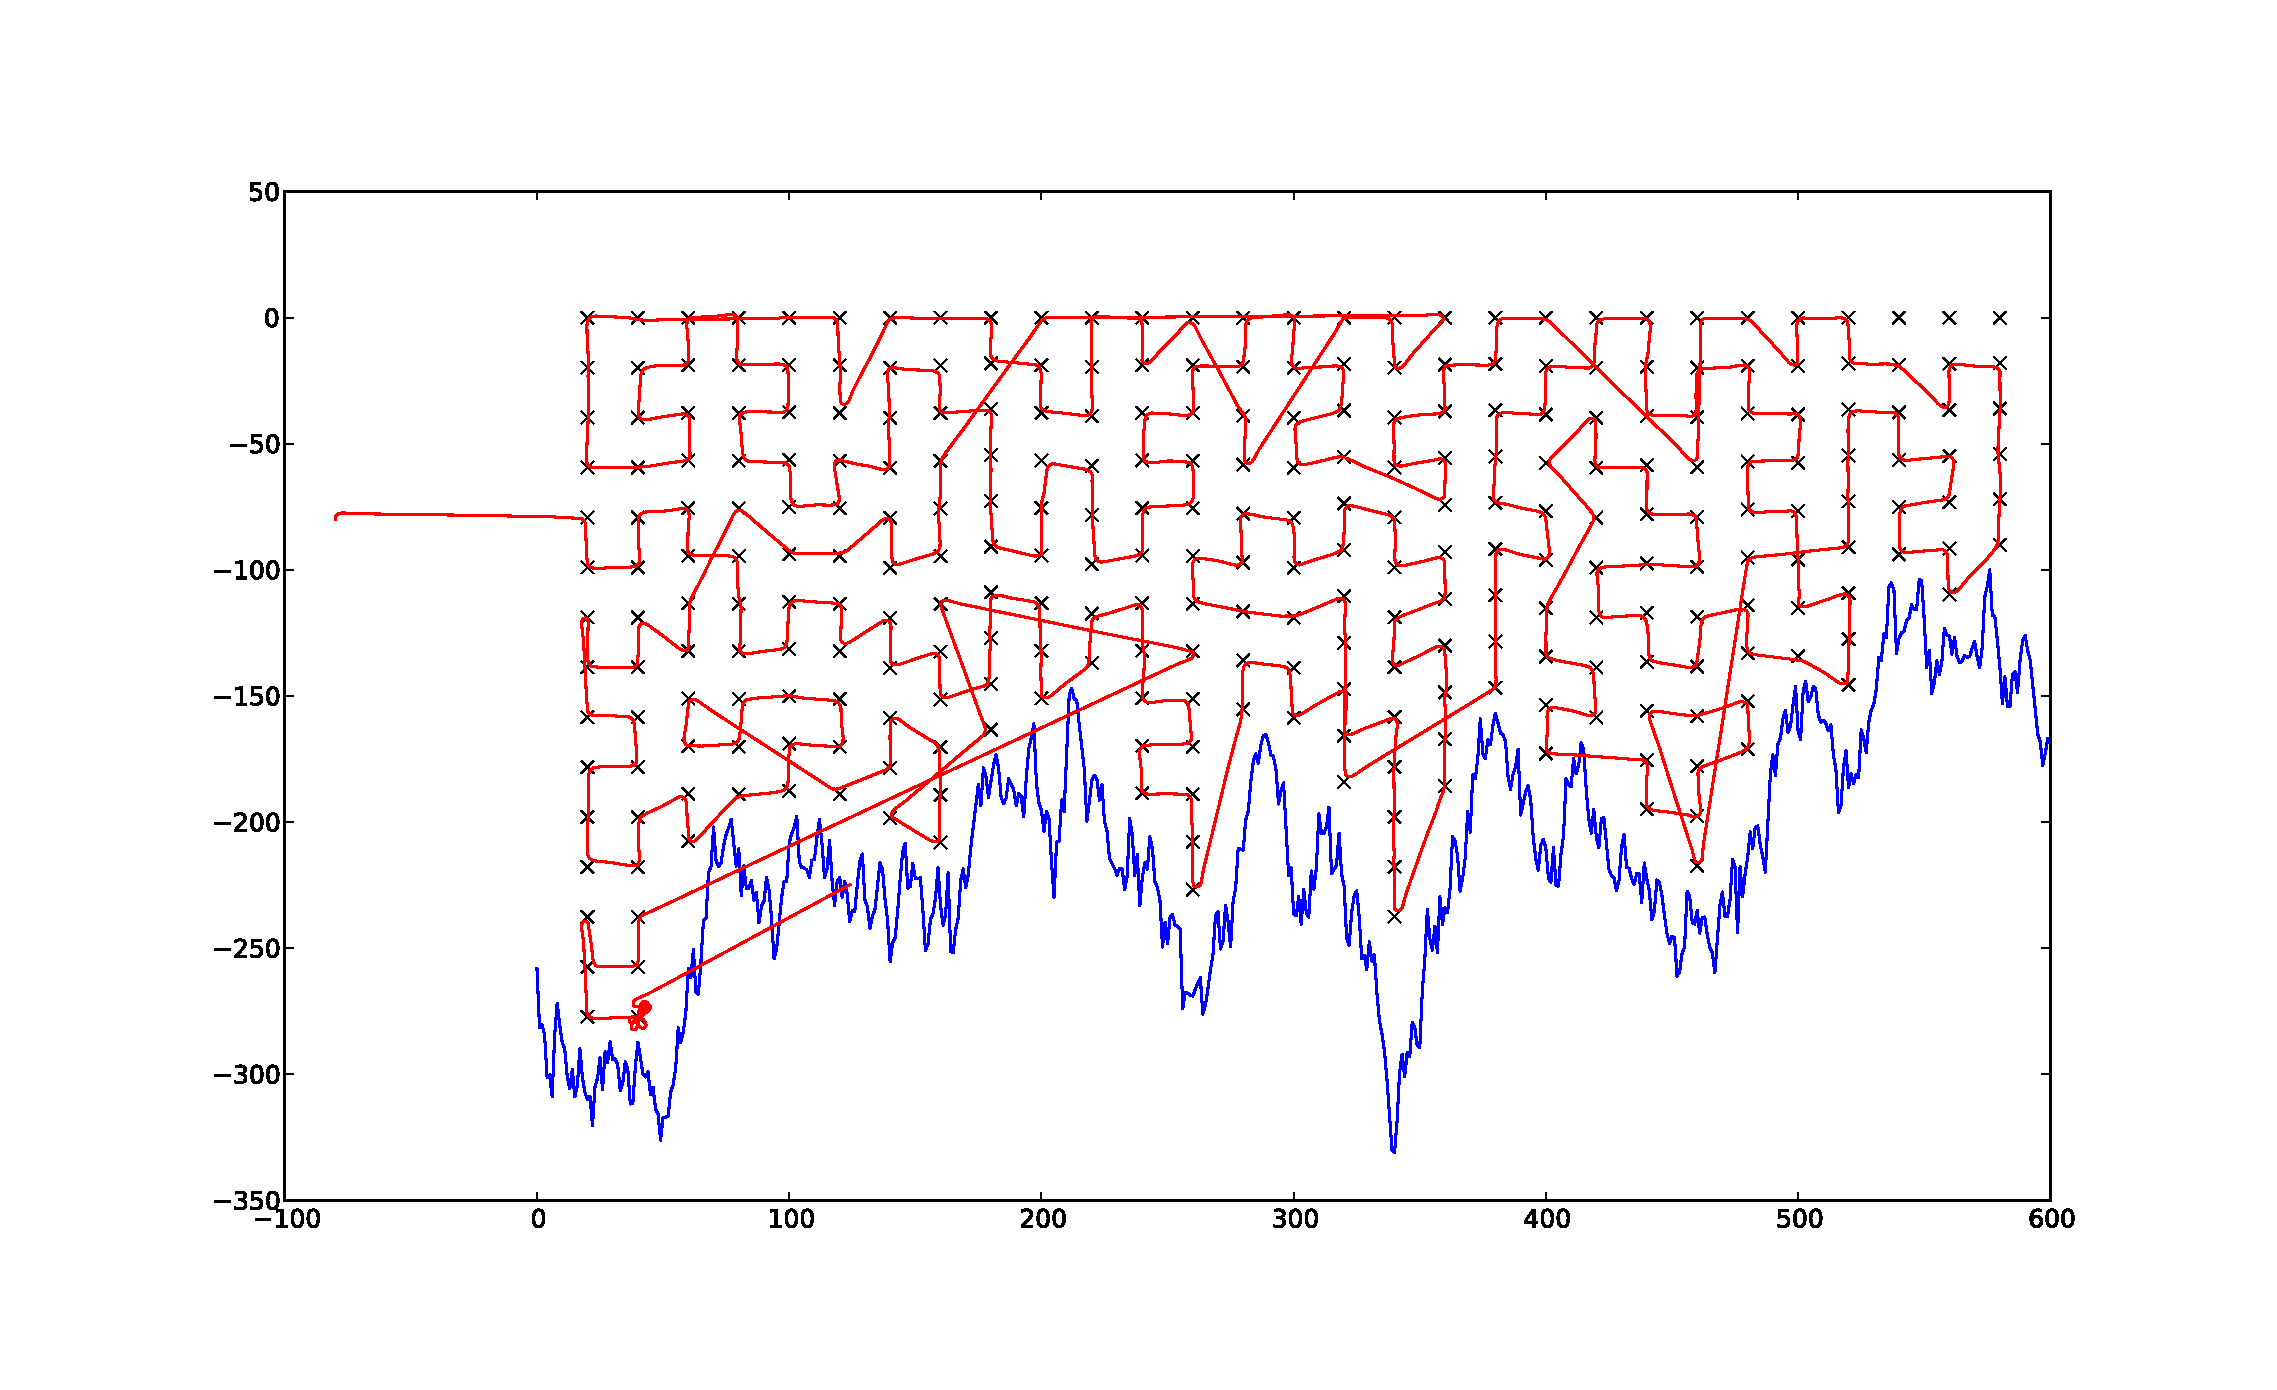
\includegraphics[width=\textwidth]{img/nn}
	\caption{Neirest neighbourgh algorithm}
	\label{fig:nn}
\end{figure}

\subsection{Lowest cost heuristics}

Even without major nautical engineering skills the following presumption can be made: If there are two paths with identical start and finish and identical lengths (start != finish) the  path with less turning is more effective.
This presumption can be extended to the following theory:

The most effective nautical path between two given points is the one with the least sum cost. The sum cost is the traveled distance times distance cost, plus absolute turnining times turning cost.

\begin{align}
	\Sigma C  = dist*C_{dist} + |turn| * C_{turn}
\end{align}

The cost of the distance and the turning depends on the type of the ship. A large, deep draught cargo ship capable of low speed will have a much higher $\frac{Distance}{Turn}$ cost ratio than a narrow military cruiser.


Using the considerations above a cost based nearest neighbour algorithm is introduced, where the lowest distance is replaced with lowest cost. The algorithm checks every point to determine which is the cheapest destination. To avoid path-loops in the map, the waypoints already visited are stored in a list. If the examined point is already in the list, the cost is increased with a redundancy value, so the algorithm will chose a different, slightly more expensive, but still unvisited measurement point. The algorithm also checks, if the path leading to the examined waypoint is clear of obsticles.

Running the simulation with the above pathplanner results in the following course: Figure~\ref{fig:lc}.

\begin{figure}[H]
	\centering
	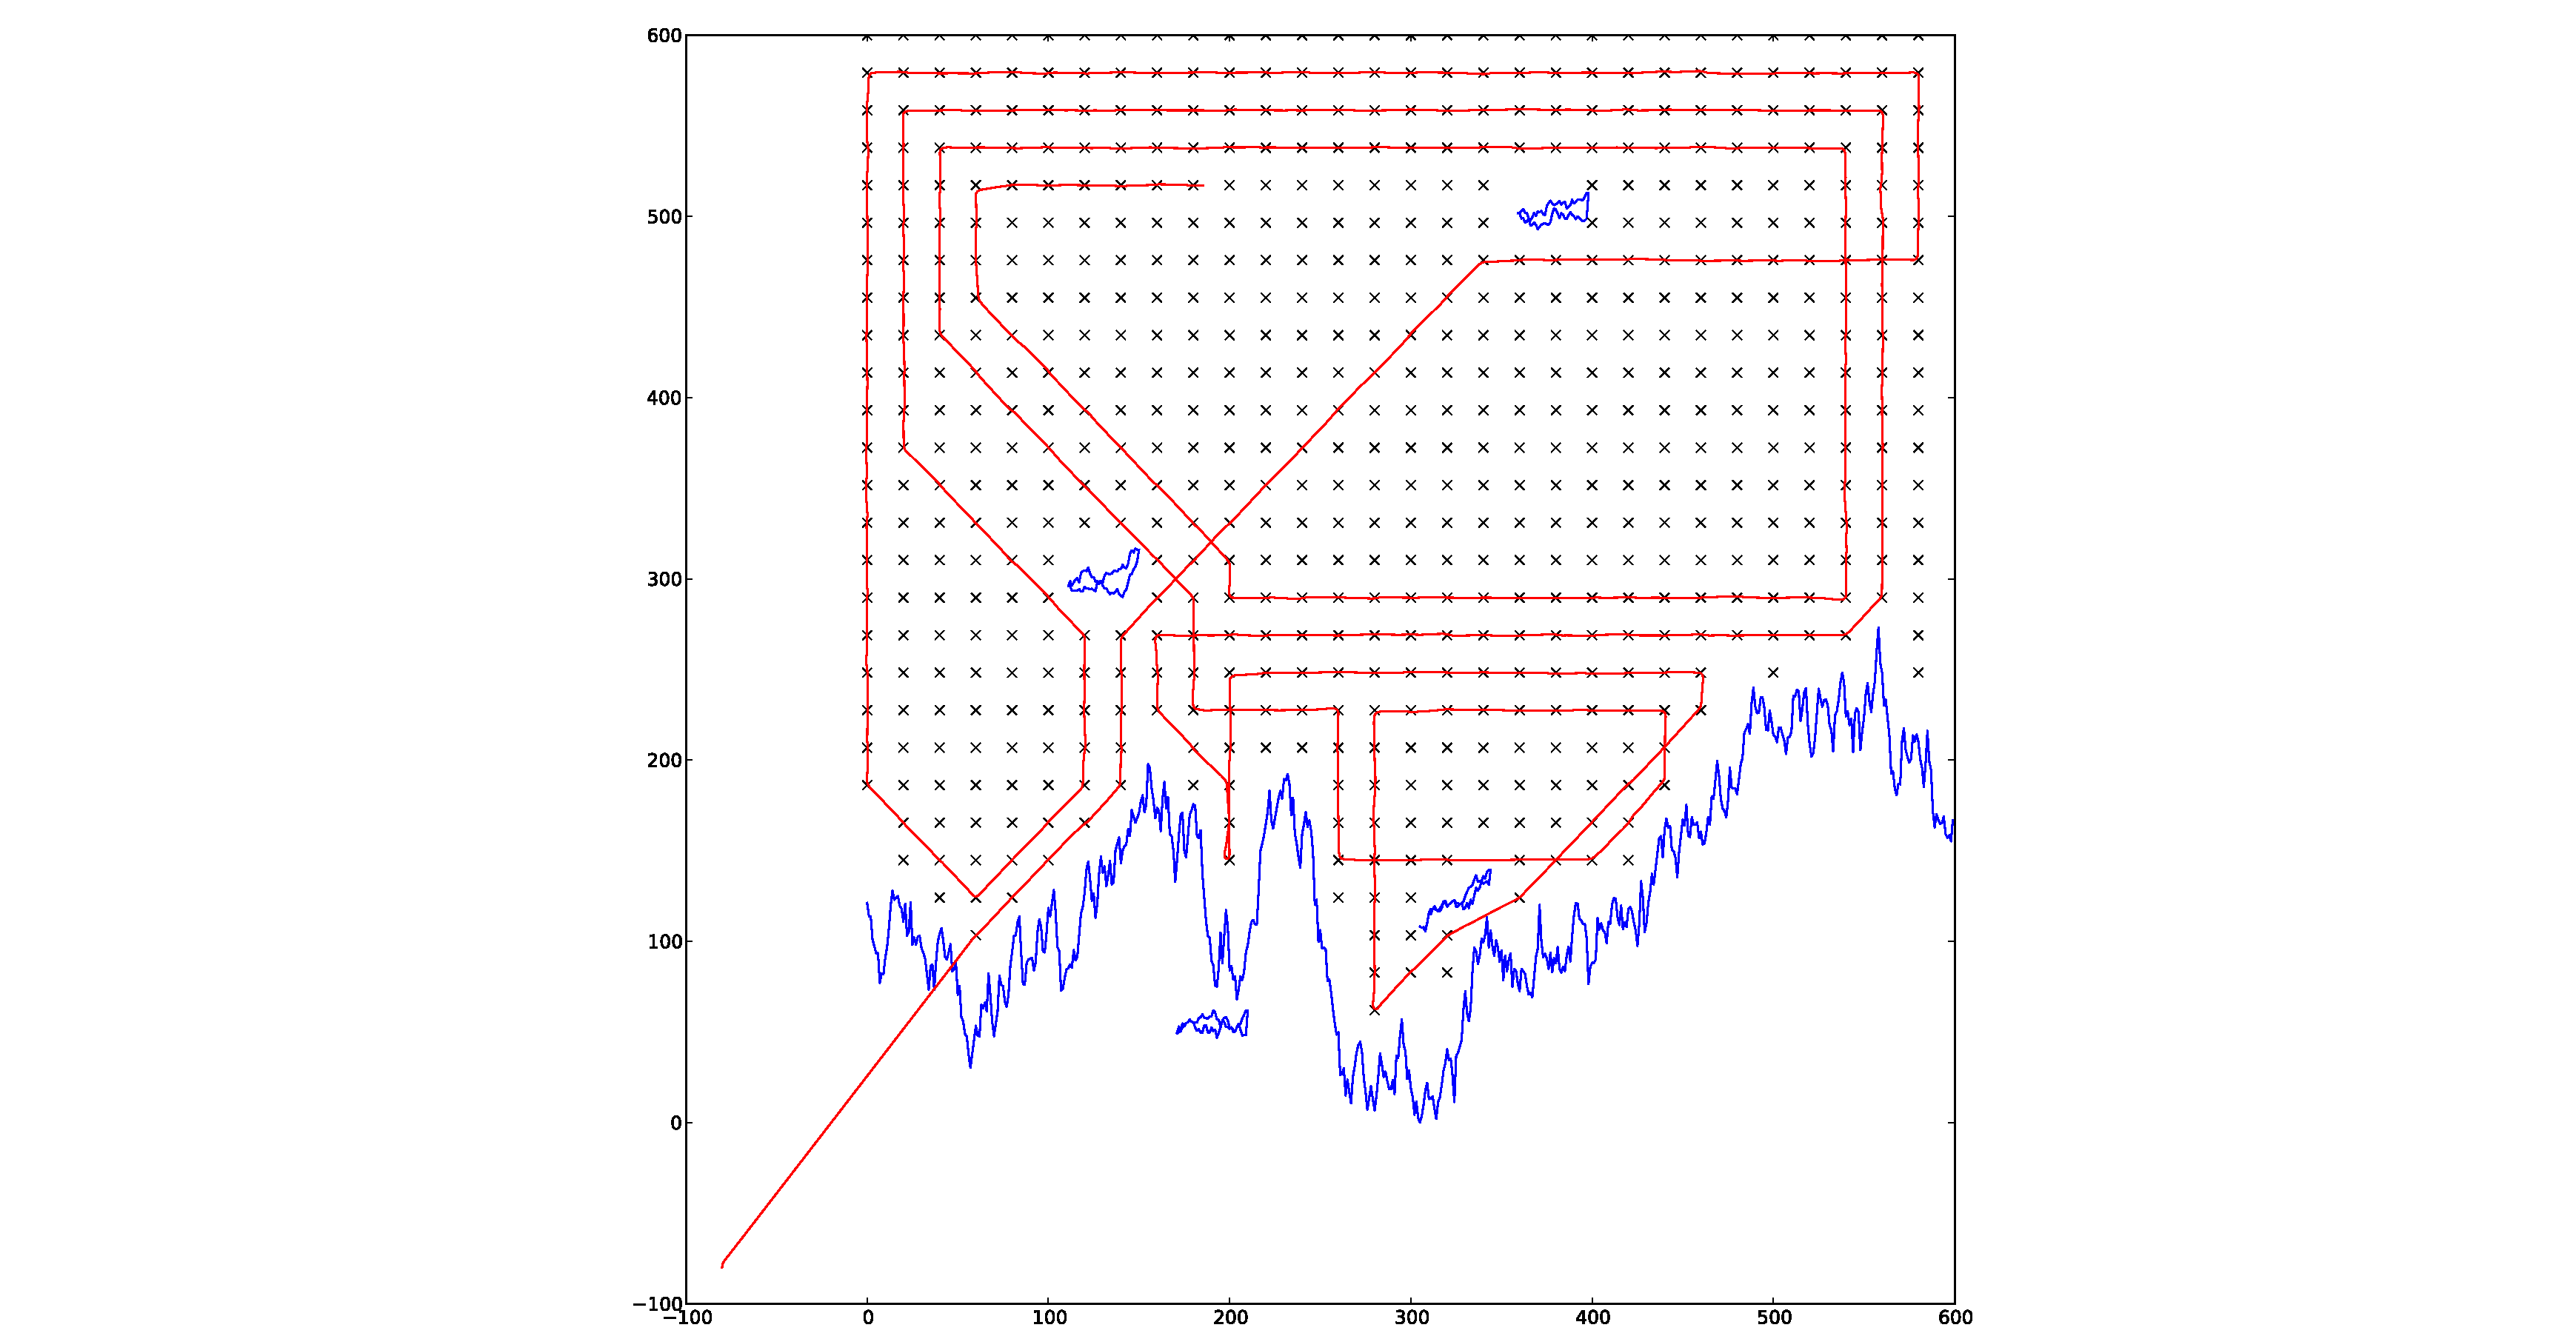
\includegraphics[width=\textwidth]{img/geee}
	\caption{Lowest cost algorithm}
	\label{fig:lc}
\end{figure}

This navigation method works adequatly in open environments. However, if the map is consisted of tight narrows and hard to navigate areas, the algorithm above fails to exit certain areas of the map. To be able to operate in such shores, a different kind of routing is required.

I call this method "Ripple", because the points examined are moving away from the surface vessel in a circular shape (well, in a rectangular actually) like a ripple. The ripple checks every neighbouroing waypoint, that wasnt checked so far, and stores the previous life of the ripple. If a point is found that has not been visited before, a list of waypoints are returned, and the ship will sail through them, and reach the destination.

Figure~\ref{fig:ripple} illustrates this navigation method by simulating a task on the map of the Earth.

\begin{figure}[H]
	\centering
	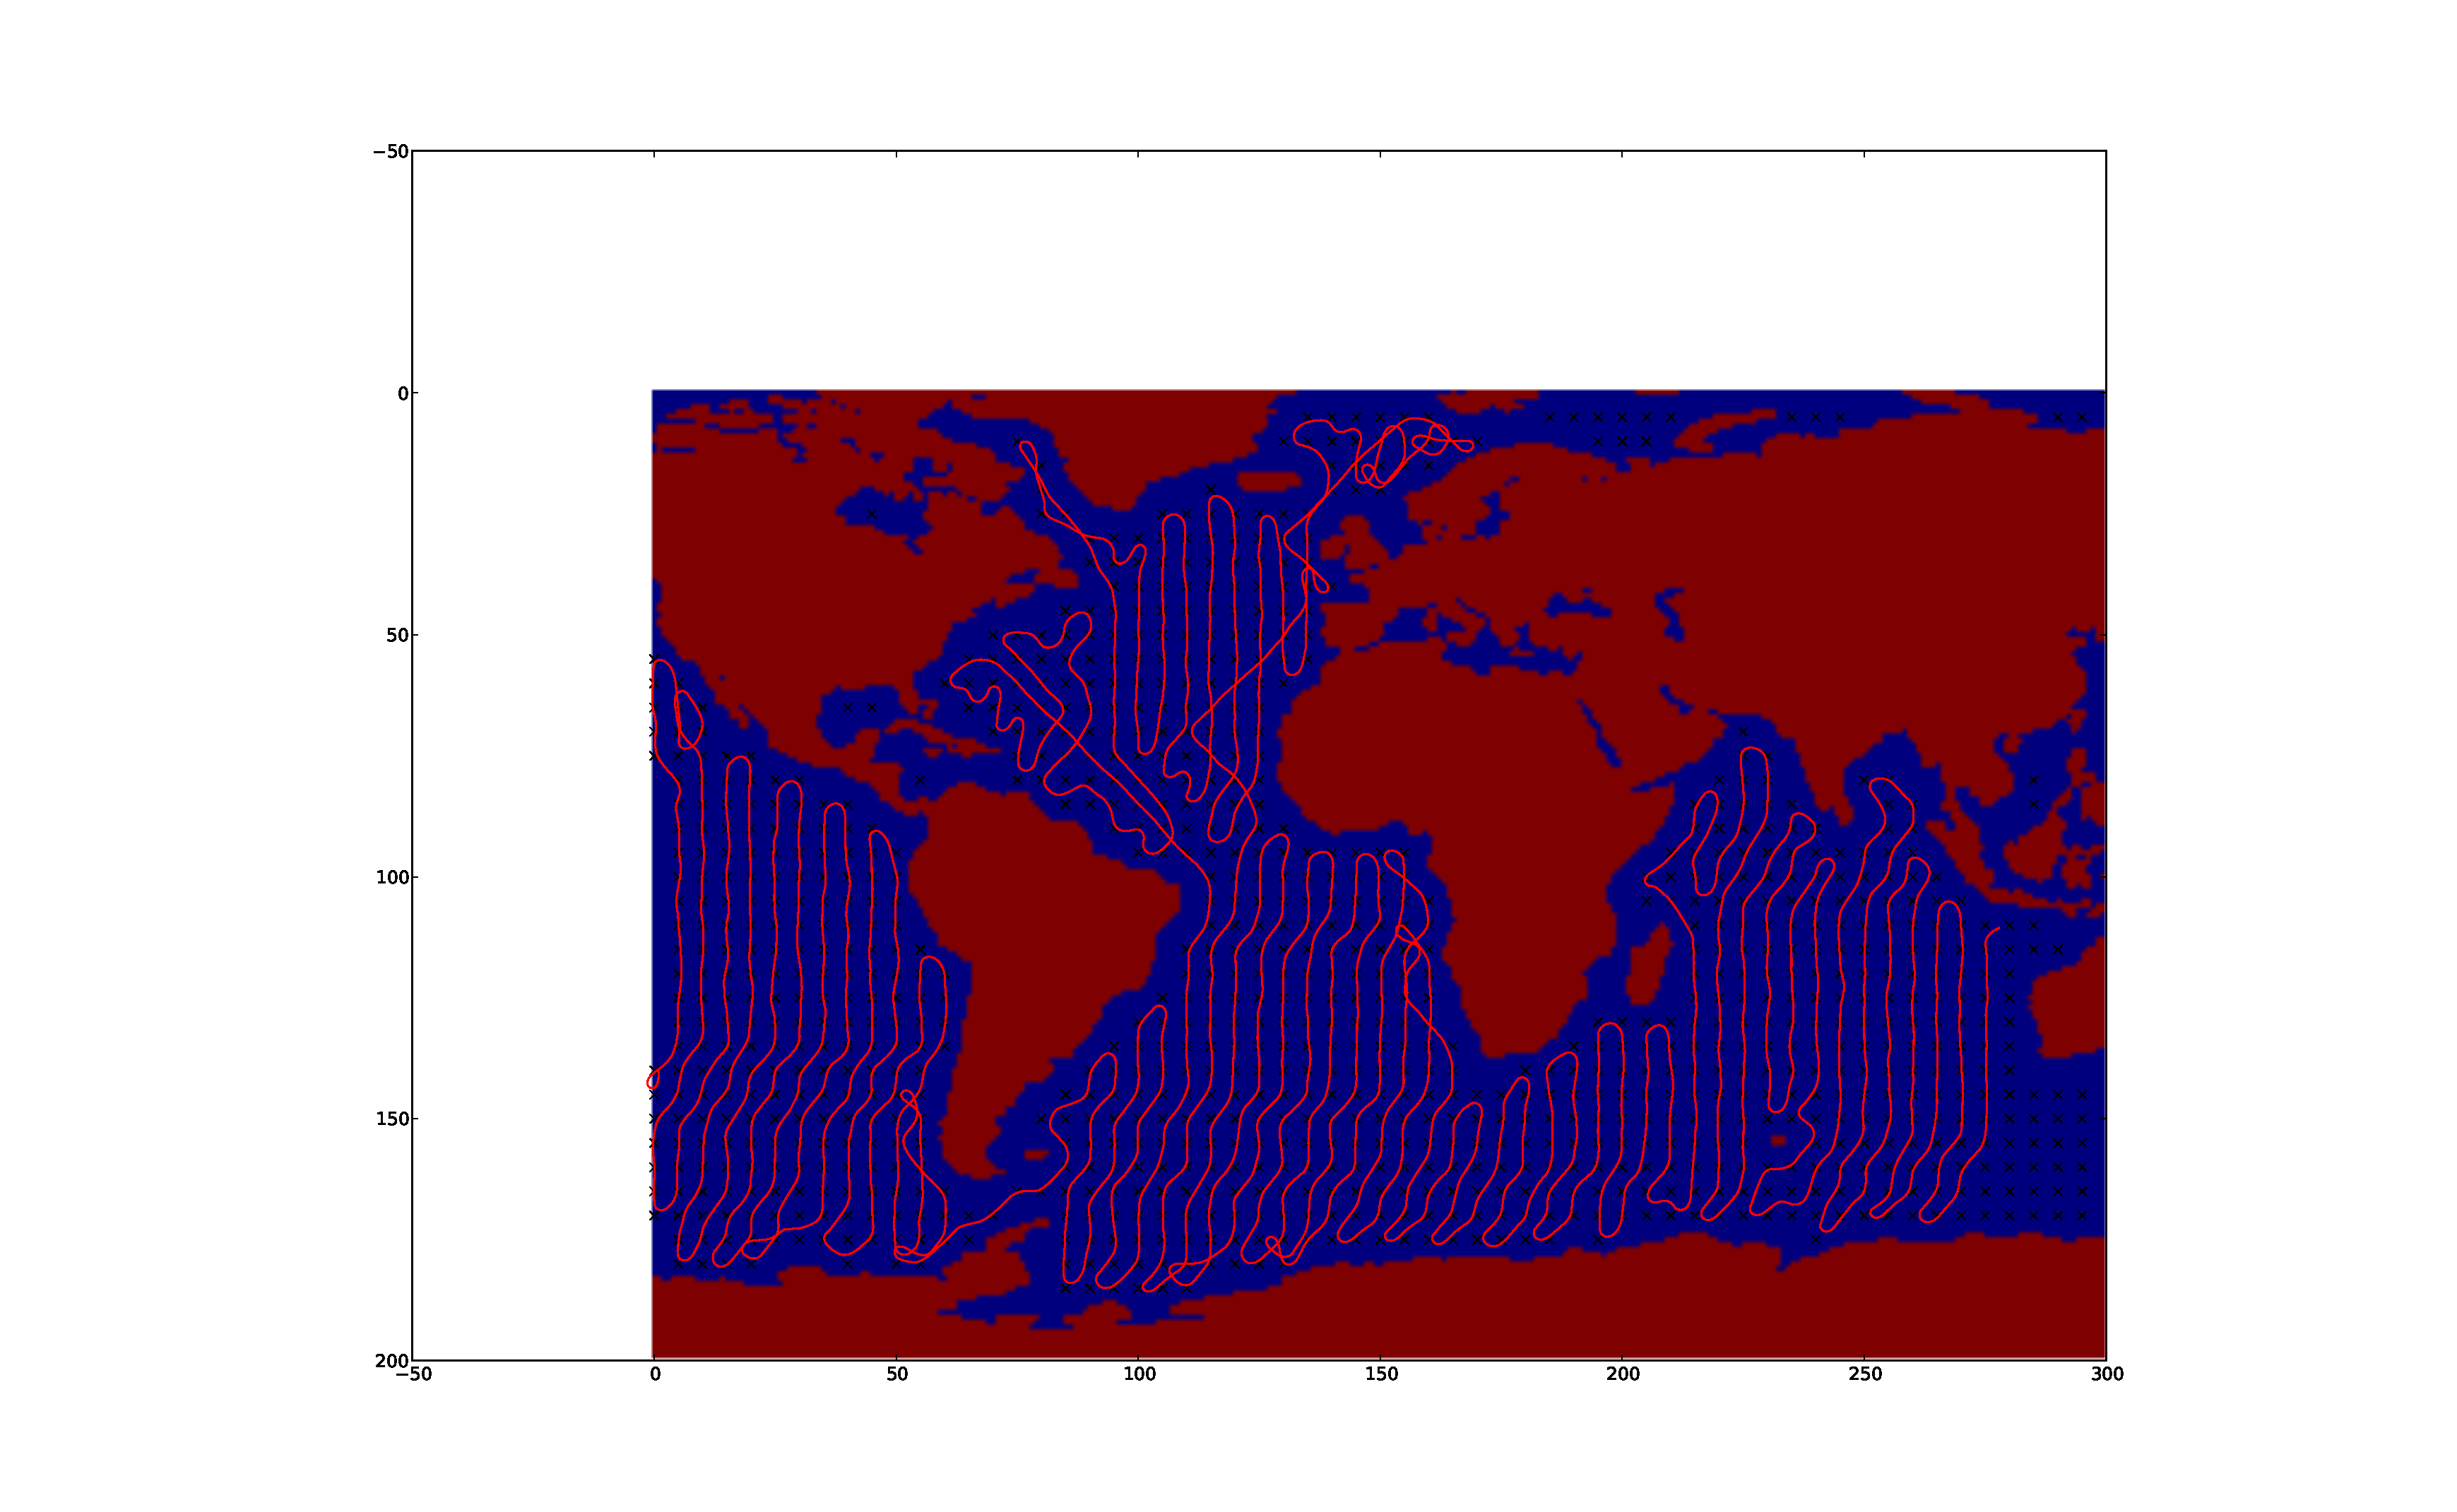
\includegraphics[width=\textwidth]{img/ripple}
	\caption{Ripple routing algorithm}
	\label{fig:ripple}
\end{figure}

\section{Navigation}

Once the required course has been set, the control system will take over the handling of the ship. The Navigation is the first and highest layer of control in the High Level Controller. In order to explain the navigation, the coordinate systems must be defined first.

\subsection{Frames of reference}

The operator team and the GPS sensor are using the Earth Centered Earth Fixed (ECEF) coordinate systems. Navigation on a spherical surface would introduce a lot of unnecessary calculations in every control cycle, since a plane can be fit onto the surface with minimal error, because the small vessel has limited maximum range.

During the Navigation the North East Down coordinate system is used to determine the attitude and position of the ship. The NED coordinate system is centered to the first GPS measurement coordinate.

A third Body Frame is also defined, the dynamic system of the ship was calculated in this frame.

\begin{figure}[H]
	\centering
	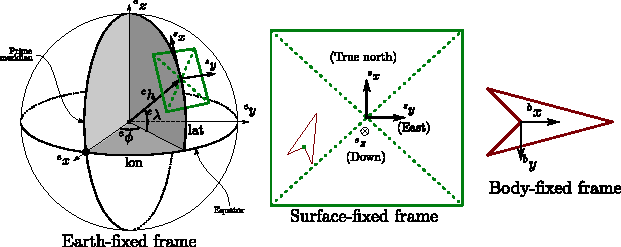
\includegraphics[width=\textwidth]{img/reference_frames}
	\caption{Used coordinate systems}
	\label{fig:coordinatesystem}
\end{figure}

\begin{align}
	\lambda = longitude  \quad \phi = latitude
	\\ GPS_{[\lambda , \phi , h]} \Longleftrightarrow [X_{NED}; Y_{NED}; Z_{NED}]
\end{align}

\subsection{Required heading}

The heading of the ship is defined in NED coordinate system. The required heading is determined by the Law of Cosines, based on the Position of the Ship and the Position of the next Sub-Waypoint.
\begin{center}

\includegraphics[scale = 0.4]{img/Law_of_Cosines}
\end{center}
Problems rise and corrections are necessary, if the heading of the ship $\theta$ is $\theta < -\pi$ or $\theta < \pi$. The heading of the ship is calculated based on the Gyro sensor and the heading can have any value in the form of: 
\begin{align}
\theta = [-{\pi} ; \pi ] \pm 2 \cdot k \cdot \pi
\end{align}\\

\begin{tcolorbox}[colback=cyan!5,colframe=cyan!40!black,title=Code: FunctionLibrary.py \\ https://www.dropbox.com/s/7nx7helisvss21a/FunctionLibrary.py]
\begin{minipage}{0,6\textwidth}
Some functions required by the software are general parametric mathematical functions, which can not be connected to any object. These functions, like the Law of Cosines, and the distance calculator function can be found in the Function Library.
\end{minipage}
\begin{minipage}{0,35\textwidth}
\raggedleft

\includegraphics[width=0.8\textwidth]{img/functionlibrary}
\end{minipage}


\end{tcolorbox}

Before invoking the control procedure, all of the heading angles must be transformed into the $[-\pi ; \pi]$ interval.
This procedure causes a possible error though.

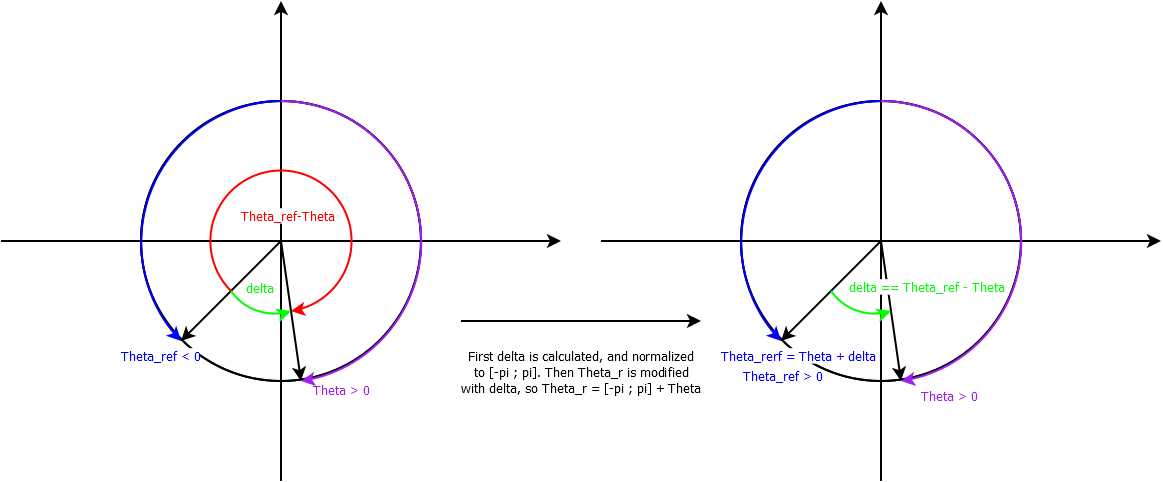
\includegraphics[width=\textwidth]{img/Headings}

The required heading or the heading of the ship must be transformed into a different representation, where 
\begin{align}
|\theta_{r}-\theta| < \pi
\end{align}
To keep a consistent heading representation, first the deviation angle 
\begin{align}
\theta = \pi_{r}-\pi
\end{align} is calculated, than transformed to the $[-\pi;\pi]$ interval and finally, with $\delta$ we can transform $\theta_{r}$ to 
\begin{align}
\theta_{r}(\theta) = \theta + \delta
\end{align}
If the conditions above are met, $\theta$ and $\theta_r(\theta)$ will always yield values that result in correct controller output.

\section{Simulator}
In order to test the generated path and eliminate some hazards of potential design errors or malfunctions, a seamless simulator is required that simulates the behaviors of the ship. \\

\begin{tcolorbox}[colback=cyan!5,colframe=cyan!40!black,title=Code: Simulator.py \\ https://www.dropbox.com/s/agron9anslev6xw/Simulator.py]
\begin{minipage}{0,6\textwidth}
According to the guidelines of the seamless simulator, this part of the system has its own distinctive object. Everything related to the simulator and everything that is unknown during the mission is stored and handled here.
\end{minipage}
\begin{minipage}{0,35\textwidth}
\raggedleft

\includegraphics[width=0.8\textwidth]{img/simulatorcode}
\end{minipage}
\end{tcolorbox}

\subsection{Requirements of the simulator}

The simulator developed for the project must meet the following conditions, otherwise the simulation might return false results, misguiding the whole development process.
\begin{itemize}
	\item The software controlling the simulated system must be unaware of the simulation
	\item The control software must be completely independent of the simulator, its variables and its functions
	\item The control software can communicate only through the same channel, as it would during normal operation
	\item Any parameters and states that are not known, only measured (e.g.: measured position != actual position) must be stored in the simulator, and must not be accessed directly from the control software
\end{itemize}

To fulfill the requirements above, the following simulator has been implemented:

\begin{figure}[H]
	\centering
	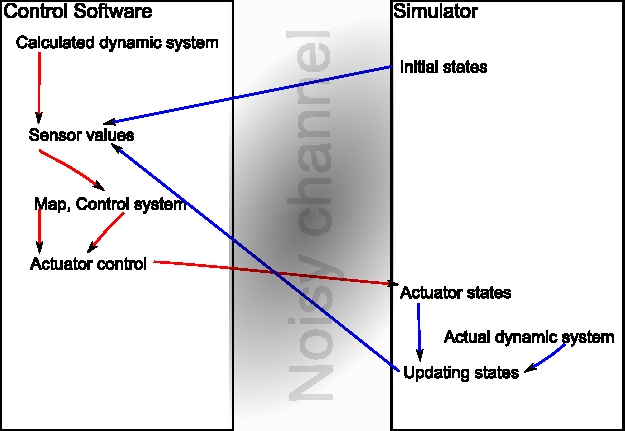
\includegraphics[width=\textwidth]{img/simulator}
	\caption{System simulator}
	\label{fig:simulator}
\end{figure}
\part{Project Laboratory II.}
\setcounter{section}{0}

It was shown in Part I. that the control software can fulfill its requirements, it's time to step forward and prepare the surveying platform: the BMESHIP.









\section{Overcoming the limitations and inaccuracies}

Unfortunately the number and quality of the available measurements is low. The different systems has their different limitations and possibilities, so does most of the actuators and motors.





\subsection{Localization and tracking}



\section{Conclusion}
This document is meant to succeeds my previous work\cite{aau}. Several major functionalities have been added, and the engine behind under the hood has been changed, and will keep changing.

My most important observation during the Project Laboratory I. was that the perceived significance of the system components might differ from the reality. The successful implementation of the different pathplanning systems and navigation required a very solid and relatively simple Map object, that can be relied on.

With the major components of the HLC now complete, up and running, it's possible to move to the next phase. In Project Laboratory II. the LLC will be designed, the communication protocol between the objects and the ship itself, in order to accomplish a more-or-less working prototype by the end of 2013.

\begin{thebibliography}{9}

\bibitem{trieste}
  Brand, V:
  \emph{Submersibles - Manned and Unmanned}\\
  South Pacific Underwater Medicine Society Journal 7 (3), 1977\\
  ISSN 0813-1988
  
 \bibitem{oceanography}
  Robert H. Stewart:
  \emph{Introduction To Physical Oceanography}
  Department of Oceanography, Texas A \& M University

\bibitem{talbot}
  Arthur Newell Talbot:
  \emph{The Railway Transition Spiral}\\
  Engineering News Publishing Company, 1901

\bibitem{kissb}
  Istv\'an Koml\'osi and B\'alint Kiss:
  \emph{Mobilis robotok auton\'om navig\'aci\'oja mozg\'o akad\'alyok elker\"ul\'es\'evel (Motion planning for multiple mobile robots using time-scaling)}\\
  InTech Open Access Publisher, 2011. pp. 259-288.\\
  ISBN: 978-953-307-842-7
  
\bibitem{aau}
	Rasmus L. Christensen, Frederik Juul, Nick \O stergaard, Tudor Muresan, Attila Fodor:
	\emph{Centralized State Estimation of Distributed Maritime Autonomous Surface Oceanographers}\\
	Section for Control and Automation, Department of Electronic Systems, Aalborg University, Denmark, 2013.
	
\bibitem{uav}
	
	\emph{Operational Requirements Document for the Unmanned Aerial Vehicle Tactical Control System Version 5.0}
	The Charles Stark Draper Laboratory Cambridge, MA 02139
	
\bibitem{res:FNPP}
	Avichal Mehra, Zulema Garraffo, Hae-Cheol Kim, Ilya Rivin, Todd Spindler, Hendrik Tolman and Ming Ji
	\emph{Ocean Plume and Tracer Modeling for the Fukushima Dai'ichi Event at NOAA}
	NCEP/NWS/NOAA Camp Springs, U.S.A.


\end{thebibliography}

\end{document}
